\subsection{Descripción del problema.}

\vspace*{0.3cm}

Este problema trata sobre distribuir $N$ productos en $C$ camiones, minimizando
el valor de $C$. Al combinarse los elementos, se obtienen distintos niveles de peligrosidad.
Para minimizar $C$, se debe tener en cuenta que contamos con un umbral de peligrosidad
$M$, \textbf{el cual no debe ser superado por la suma de los niveles de peligrosidad de los
elementos que contiene}.

\vspace*{0.5cm}

\textbf{Ejemplo:}
\begin{itemize}
  \item Dado $M = 7$ y 4 productos $p_1, p_2, p_3$ y $p_4$, con una relación
  de peligrosidad $h_{1,2} = 5, h_{1,3} = 3, h_{1,4} = 4, h_{2,3} = 6, h_{2,4} =
  3$ y $h_{3,4} = 5$, la solución óptima es utilizar 2 camiones, el primero
  transportando $p_1$ y $p_3$, y el segundo transportando $p_2$ y $p_4$.
\end{itemize}



\subsection{Desarrollo de la idea y pseudocódigo.}

Para resovler el problema, empezamos utilizando un solo camión e intentamos ubicar
todos los elementos en el mismo. De no ser posible, se agrega otro camión y se vuelven
a intentar todas las combinaciones de elementos en los mismos. Si siguen sin caber los
elementos, se agrega un camión más y se vuelve a empezar.

Este proceso continúa hasta encontrar una cierta cantidad de camiones, capaz de
transportar todos los elementos. Por la estrategia planteada para el problema,
\textbf{la solución encontrada será una solución óptima}.

\vspace*{0.5cm}


\begin{codebox}
\Procname{$\proc{biohazard}(elementos, maximaPeligrosidad)$}
\li $\id{camiones} \gets []$
\li $\proc{agregar}(camiones, camion)$
\li \While $(\neg\proc{backtracking}(camiones, elementos))$
\li     \Do
            $\proc{agregar}(camiones, camion)$
        \End
\li \Return $\id{camiones}$
\end{codebox}


\vspace*{0.5cm}


\begin{codebox}
\Procname{$\proc{backtracking}(camiones, elementos)$}
\li \If $\proc{vacio?}(elementos)$
\li     \Then
            \Return $\const{true}$
        \End
\li $\id{elemento} \gets \proc{dameUno}(elementos)$
\li $\id{elementos} \gets elementos \setminus \{elemento\}$
\li \For $camion \in camiones$
\li     \Do
            \If $\proc{entra?}(elemento, camion)$
\li             \Then
                    $\proc{agregar}(camion, elemento)$
\li                 \If $\proc{backtracking}(camiones, elementos)$
                        \Then
\li                         \Return $\const{true}$
\li                 \Else
\li                     $\proc{borrar}(camion, elemento)$
                    \End
            \End
        \End
\li $\id{elementos} \gets elementos \cup \{elemento\}$
\li \Return $\const{false}$
\end{codebox}



\newpage
\subsection{Análisis de complejidad.}

\vspace*{0.3cm}


La función \verb|backtracking| es llamada desde la función \verb|biohazard|, en
el peor de los casos, tantas veces como elementos haya para insertar en los camiones.
Una vez que se comienza a hacer la recursión, por cada camión que podemos utilizar,
se vuelve a hacer con un elemento menos. La recursión finaliza en el momento en
el que se la invoca con un conjunto vacío de elementos. Como la cantidad de
elementos siempre disminuye en 1 con cada llamado recursivo, en $n$ llamados se
corta la recurrencia.

En el peor de los casos, cuando nos veamos obligados a recorrer
todos los árboles de decisiones, al intentar poner los productos en un
camión, tendremos un árbol $1$-ario de altura $n$. Al hacerlo con 2
camiones, tendremos un árbol $2$-ario de altura $n$, pero sabemos que los
productos no entran en un camión y el algoritmo nunca intentará poner los
$n$ elementos en un solo camión. Por lo tanto, la altura de este árbol será
de $n - 1$. Generalizano, al intentar distribuir los $n$ productos en $k$
camiones, tendremos un árbol $k$-ario de altura $n - k + 1$.

La complejidad del algoritmo va a ser la suma de todos los nodos sobre
los árboles de decisiones. Dicho de otro modo, la complejidad será

\begin{align*}
  O(\sum_{k=1}^n k^{n - k + 1})
\end{align*}

\vspace*{0.75cm} \noindent


\newpage
\subsection{Experimentación y gráficos.}

\vspace*{0.3cm}

\subsubsection{Test 1 - benchmark caso aleatorio}

(ver \verb|info.3.dat|) \medskip

En este test, tenemos $n$ elementos en cada instancia, con $n$ inicializado en 1 e incrementándose
también en 1 hasta alcanzar 20 y un umbral $m$ de peligrosidad, que se inicializa en 2 y se incrementa
en 2 en cada instancia, hasta alcanzar el valor 40.

Para cada instancia, se toma el \textbf{valor mínimo} de cantidad de ciclos luego de \textbf{20 corridas}.

\vspace*{0.5cm}

\begin{figure}[h]
  \begin{center}
    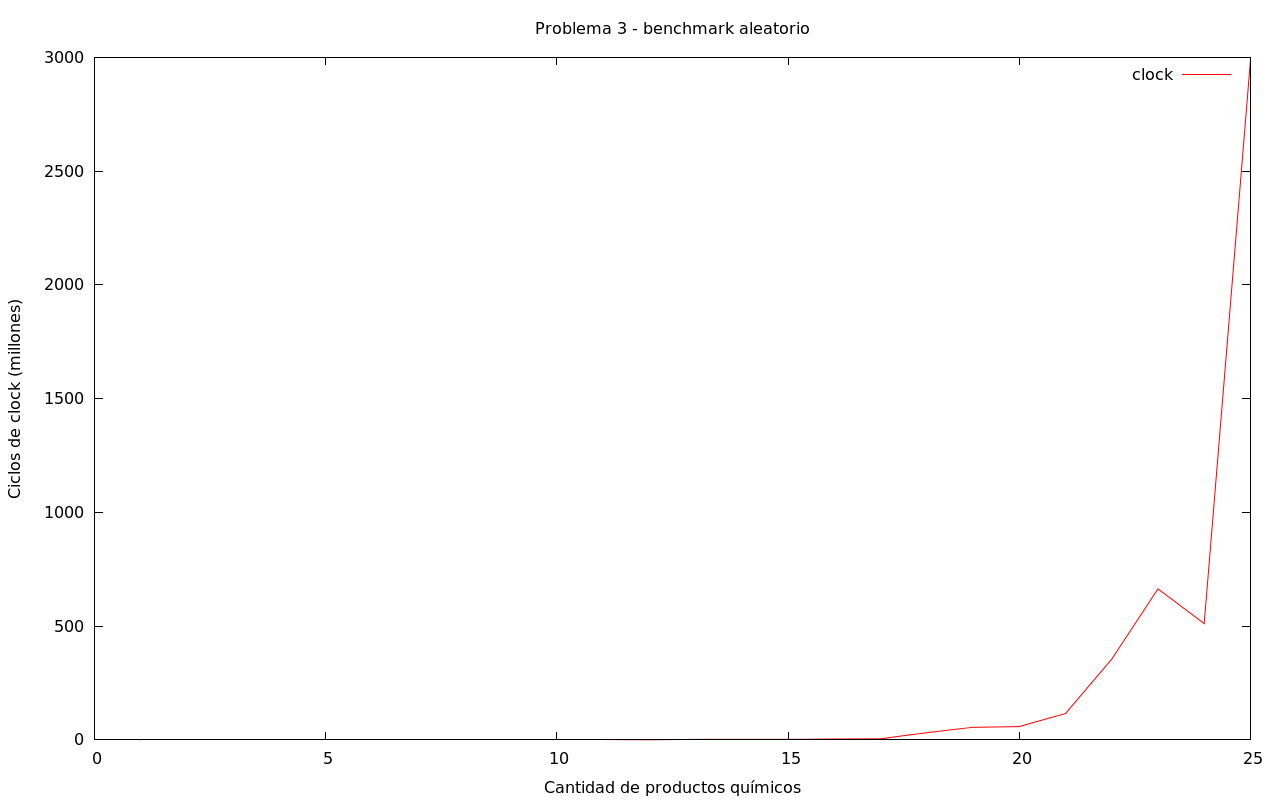
\includegraphics[scale=0.35]{imagenes/grafico-3.png}
  \end{center}
\end{figure}

\vspace*{0.5cm}

En este gráfico podemos apreciar que el comportamiento del algoritmo es
sumamente aleatorio en el caso promedio. Esto se debe a la naturaleza poco
predecible del mismo, ya que en base a cómo sean los valores de entrada, las
podas se realizan en momentos diferentes.


\newpage
\subsubsection{Test 2 - benchmark del peor caso}

(ver \verb|info.3.peor.dat|) \medskip

\underline{\textbf{NOTA:}} para el peor caso redujimos la cantidad de instancias a 16 por fines prácticos, dada la complejidad
del algoritmo y el tiempo de ejecución requerido para finalizar más instancias. \medskip

En este test, tenemos $n$ elementos en cada instancia, con $n$ inicializado en 1 e incrementándose
también en 1 hasta alcanzar 16 y un umbral $m$ de peligrosidad, que se mantiene constante en 0 para todas las
instancias.

Para cada instancia, se toma el \textbf{valor mínimo} de cantidad de ciclos luego de \textbf{16 corridas}.

\vspace*{0.5cm}

\begin{figure}[h]
  \begin{center}
    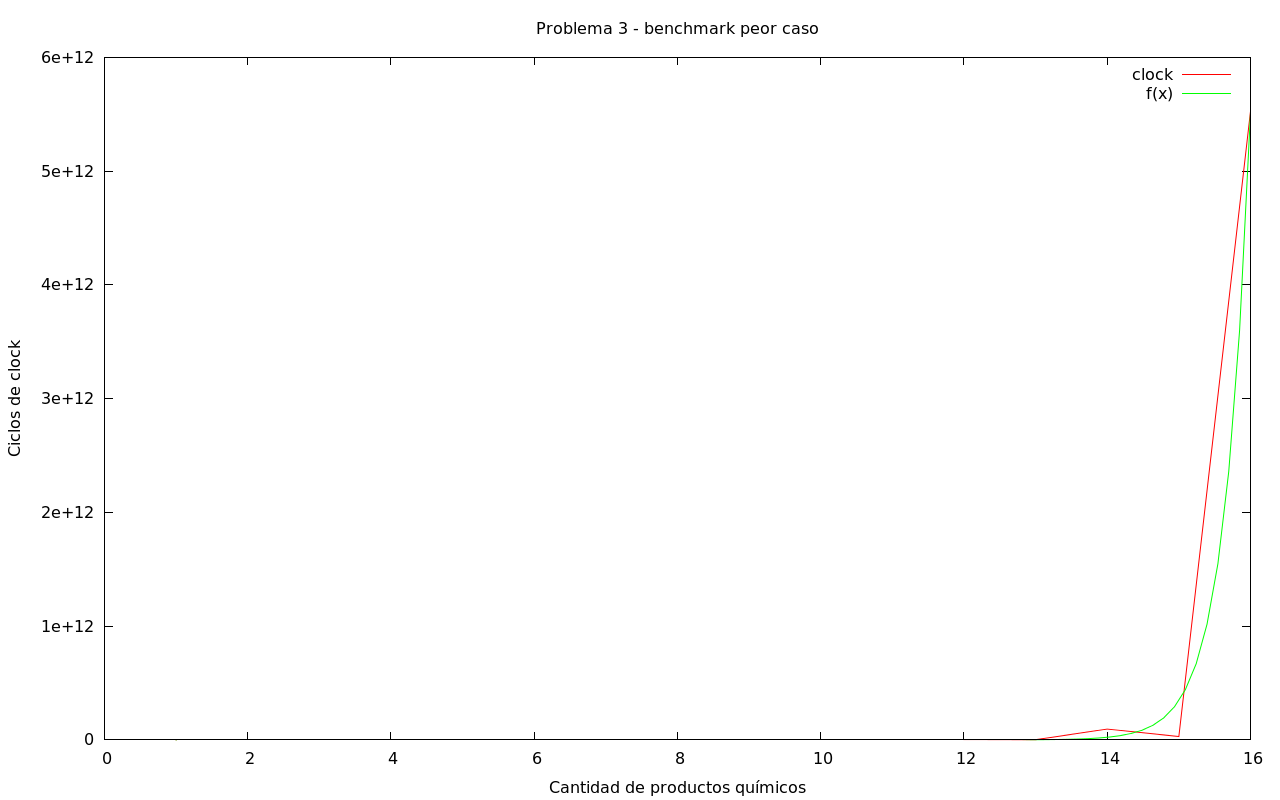
\includegraphics[scale=0.35]{imagenes/grafico-3-peor.png}
  \end{center}
\end{figure}

\vspace*{0.5cm}

En este gráfico podemos apreciar que a partir de los 10 elementos, el
crecimiento de la cantidad de ciclos de clocks necesarios para completar las
instancias crece exponencialmente, llegando a un pico de casi 6 billones de
ciclos de clock.


\newpage
\subsubsection{Test 3 - benchmark del mejor caso}

(ver \verb|info.3.mejor.dat|) \medskip

En este test, tenemos $n$ elementos en cada instancia, con $n$ inicializado en 1 e incrementándose
también en 1 hasta alcanzar 20 y un umbral $m$ de peligrosidad, que se inicializa en 1000000 y se incrementa
también de a 1000000 en cada instancia, hasta alcanzar el valor 20000000.

Para cada instancia, se toma el \textbf{valor mínimo} de cantidad de ciclos luego de \textbf{20 corridas}.


\begin{figure}[h]
  \begin{center}
    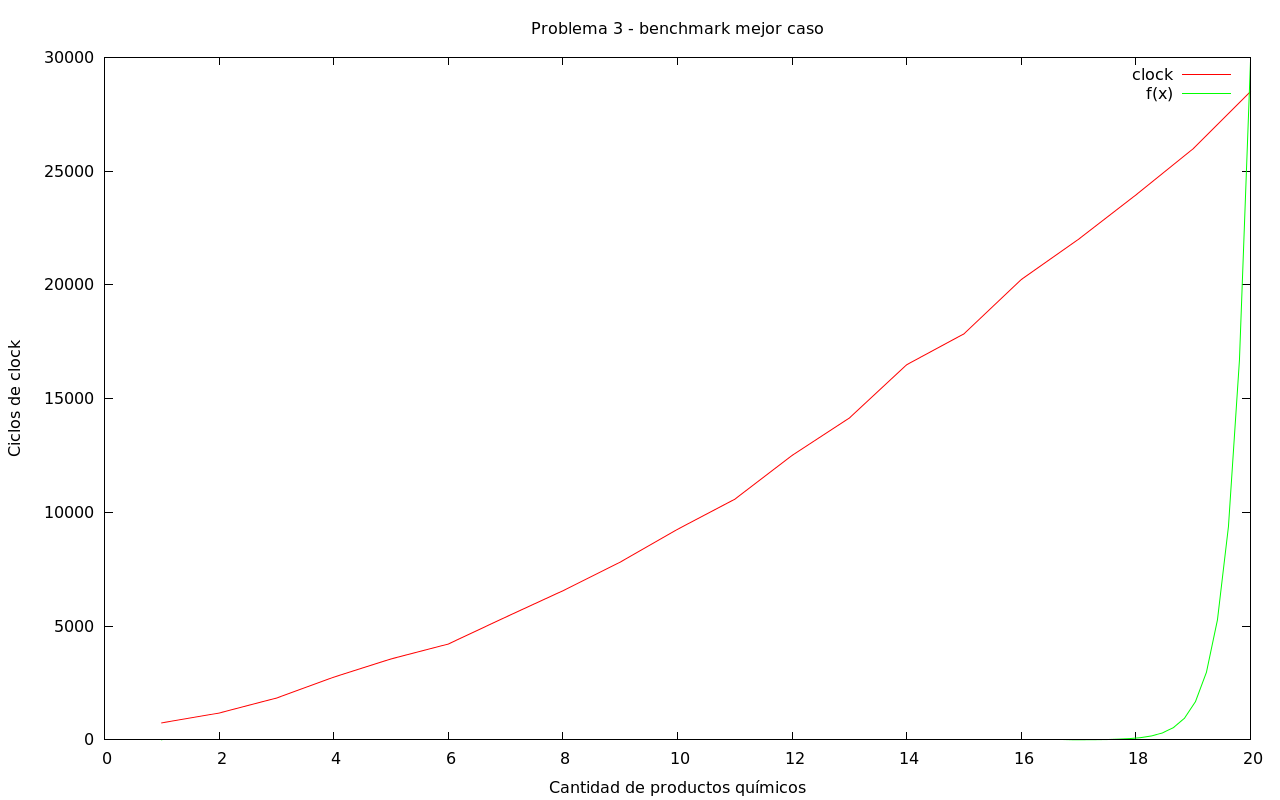
\includegraphics[scale=0.35]{imagenes/grafico-3-mejor.png}
  \end{center}
\end{figure}


En este gráfico podemos apreciar que el algoritmo, tiene un comportamieno
muy veloz en comparación contra instancias aleatorias o de peor caso. Esto
se debe a que el mismo se reduce a realizar una pequeña serie de sumas en el
caso de que todos los elementos entren en un solo camión.
